
\documentclass{article}

\usepackage{lmodern}

\usepackage[T1]{fontenc} 
\usepackage[utf8]{inputenc}


\PassOptionsToPackage{tableposition=top}{caption}

\usepackage{lwarp}
% \booltrue{HTMLDebugComments}
% \tracinglwarp

\usepackage{textcomp}

\usepackage{printlen}


\usepackage[inner=.5in,outer=2.5in,marginparwidth=2in]{geometry}

% \newgeometry{inner=.5in,outer=2.5in,marginparwidth=2in}


\usepackage{microtype}

\usepackage{lipsum}
\usepackage{blindtext}

\usepackage{xcolor}

\usepackage{graphicx}
\graphicspath{{images/}}

\usepackage{tocdata}
\tdartisttextleft

\makeatletter
\@ifpackageloaded{tocdata}{}{
    \newcommand*{\sectionauthor}[3]{\section{#1}}
}
\makeatother


% \usepackage{titletoc}
% \titlecontents{section}[3.75em]{}{\contentslabel{2.25em}}{}{%
% % \dotfill
% \titlerule*[.75pc]{.}%
% \contentspage}[\vspace{-.5ex}]%


% To test prohibited packages:
% \usepackage{subfig}
% \usepackage{subfigure}
% \usepackage{floatrow}



\usepackage{keyfloat}


\usepackage{caption}


% To test prohibited packages:
% \usepackage{subfig}
% \usepackage{subfigure}
% \usepackage{floatrow}
% \usepackage{float}
% \usepackage{floatflt}
% \usepackage{subfloat}

\usepackage{newfloat}
\DeclareFloatingEnvironment[
    fileext={lod},
    listname={List of Diagrams},
    name={Diagram},
]{diagram}


\captionsetup[figure]{
	style=default, justification=centering,
	margin=0pt, parskip=0pt, skip=1ex,
	labelfont={small,bf},textfont={small,bf}
}

\captionsetup[table]{
	style=default, justification=centering,
	margin=0pt, parskip=0pt, skip=1ex,
	labelfont={small,bf},textfont={small,bf},
    position=top
}

\captionsetup[subfigure]{
	style=default, justification=centering,
	margin=0pt, parskip=0pt, skip=1ex,
	labelfont={small},textfont={small}
}

\captionsetup[subtable]{
	style=default, justification=centering,
	margin=0pt, parskip=0pt, skip=1ex,
	labelfont={small},textfont={small},
    position=top
}

\captionsetup[diagram]{
    style=default, justification=centering,
    margin=0pt, parskip=0pt, skip=1ex,
    labelfont={small,bf},textfont={small,bf}
}


\setlength{\floatsep}{5ex plus 1ex minus 1ex}
\setlength{\dblfloatsep}{5ex plus 1ex minus 1ex}


\setlength{\parskip}{3ex}
\setlength{\parindent}{0pt}

\title{Keyfloat Test Document}
\author{Brian Dunn\\ \textsc{\footnotesize{BD Tech Concepts LLC}}}
\date{some date}


\usepackage{hyperref}
\hypersetup{colorlinks}

\usepackage{cleveref}
\crefname{diagram}{diagram}{diagrams}
\crefname{subdiagram}{subdiagram}{subdiagrams}


\newcommand{\cs}[1]{\textsf{\textbackslash#1}}
\newcommand{\env}[1]{\textsf{#1}}
\newcommand{\pkg}[1]{\textbf{\texttt{#1}}}
\newcommand{\acro}[1]{\textsc{\MakeLowercase{#1}}}

\StartDefiningTabulars
\newcommand{\testtable}{%
\begin{tabular}{cc}%
\hline\rule{0pt}{2.7ex}%
A & B \\
C & D \\
\hline
\end{tabular}%
}

\newcommand{\testwidetable}{%
\begin{tabular}{cccc}%
\hline\rule{0pt}{2.7ex}%
A & B & C \\
D & E & F \\
\hline
\end{tabular}%
}

\newcommand{\testtablethree}{%
\begin{tabular}{ccc}
\hline
a & b & c \\
d & e & f \\
\hline
\end{tabular}%
}

\StopDefiningTabulars


\setlength{\fboxsep}{5pt}
% \setlength{\FrameSep}{5pt}
% \setlength{\FrameRule}{.4pt}








\CSSFilename{testfloat.css}

\begin{document}


\maketitle

\tableofcontents
\listoffigures
\listoftables
\listofdiagrams

\clearpage

\color{blue}

\sectionauthor{Figure without a caption}{First}{Last}

The first figure is a simple figure without a caption, label, frame, or additional text.

\keyfig{}{image}

\section{Caption}

\keyfig{c=Adds a caption}{image}

The section figure adds a caption.


\section{Short Caption}

\keyfig{c={Adds a short caption},sc={Short Caption}}{image}

The third figure adds a short caption for the table of contents.


\section{Label}

\keyfig{l=fig:addlabel,c={Caption and a label}}{image}

Figure \ref{fig:addlabel} adds a label.


\section{Cleveref}

\keyfig{l=fig:cleveref,c={Cleveref}}{image}

\Cref{fig:cleveref} tests the use of the \pkg{cleveref} package.


\section{Frame}

\keyfig{l=fig:framed,c={Tightly Framed},ft}{image}

Figure \ref{fig:framed} adds a tight frame.


\keyfig{l=fig:looselyframed,c={Loosely Framed},f}{image}

Figure \ref{fig:looselyframed} adds a loose frame.


\section{Additional Text}

\keyfig{,l=fig:text,c={Additional Text},f,t={This is additional text.

With multiple lines.}}{image}

Figure \ref{fig:text} adds additional text.


\section{Linewidth}

\keyfig{,l=fig:addlinewidth,c={Half of \cs{linewidth}},f,lw=.5}{image}

Figure \ref{fig:addlinewidth} is half of \cs{linewidth}.

\keyfig[H]{c={Half of \cs{linewidth} [H]},f,lw=.5}{image}


\section{Fixed Width}

\keyfig{,l=fig:fixedwidth,c={One cm Wide},f,w=1cm}{image}

Figure \ref{fig:fixedwidth} is one centi-meter wide.


\section{Fixed Height}

\keyfig{l=fig:fixedheight,c={One cm Tall},f,h=1cm}{image}

Figure \ref{fig:fixedheight} is one centi-meter tall.


\section{Fixed Scale}

\keyfig{,l=fig:fixedscale,c={Scaled 3\texttimes},f,s=3}{image}

Figure \ref{fig:fixedscale} is scaled 3\texttimes.


\section{Rotation}

\keyfig{c={Rotated 90 degrees},f,r=90}{image2}

\keyfig{c={Rotated 30 degrees},f,r=30}{image2}


\clearpage



\section{Figures ``Here''}

% \setlength{\intextsep}{20pt}

Figure \ref{fig:here} is located here:

\keyfig[H]{,f,c={A figure [H]},l=fig:here}{image}

This figure may be out of sequence with surrounding figures.
Place a \cs{clearpage} in front to re-sync if necessary.


The following is a figure [H] without a caption:

\keyfig[H]{f,cstar={}}{image2}

Another figure [H]ere:

\keyfig[H]{,f,c={Another figure [H]}}{image}

After.


\clearpage


\section{Starred Caption}

A figure with a starred caption does not increment the \texttt{figure} counter.

\cs{thefigure} is \thefigure\ before adding the star captioned figure.

\keyfig{,f,cstar={A starred caption}}{image}


\cs{thefigure} is \thefigure\ after adding the starred captioned figure.

A starred caption does not appear in the list of figures, unless there is a short caption.


\keyfig{,f,cstar={Starred caption with an empty short caption.},sc={}}{image}

A starred caption with an empty short caption does not appear in the \acro{LOF}.

\keyfig{,f,cstar={Starred caption with a short caption.},sc={Starred short caption}}{image}

\cs{thefigure} is \thefigure\ after adding the starred short caption which appears in the \acro{LOF}.

Adding a \texttt{sc} ``short caption'' causes the short caption to appear in the
list of figures, even though the \verb|cstar| key is used.






Text before the starred [H] figure.

\keyfig[H]{cstar={Starred caption [H]}}{image2}

Text after the starred [H] figure.

\clearpage




\section{Row of Figures}


\keyfig{c=Before the keyfloats}{image2}

before
\begin{keyfloats}{2}
\keyfig{lw=1,f,c={First in a group},l=fig:firstinrow,t={\raggedright \cs{raggedright}}}{image}
\keyfig{lw=1,f,c={Second in a group},l=fig:secondinrow,t={\raggedleft \cs{raggedleft}}}{image2}
\begin{keyfloats}{2}
\keyfig{f,lw=1,c={Third in a group}}{image}
\keyfig{f,lw=.5,c={Fourth in a group}}{image2}
\keyfig{,lw=1,c={Fifth in a group}}{image}
\keyfig{lw=1,c={Sixth in a group}}{image2}
\end{keyfloats}
\keyfig{lw=.5,c={Seventh in a group},l=fig:seventhinrow}{image2}
\end{keyfloats}
after the keyfloats

\Crefrange{fig:firstinrow}{fig:seventhinrow} are in a \env{keyfloats} environment.

\clearpage




\section{Subfigures}

before
\begin{keysubfigs}{3}{c=Sub-Figures,l=fig:subfigs}
\keyfig{lw=1,f,c={First Subfigure},l=fig:firstsubfig,t=Some Text}{image}
\keyfig{lw=1,f,r=90,c={Second Subfigure},l=fig:secondsubfig,t=Lots of lots of lots of lots of text.}{image2}
\begin{keyfloats}{1}
\keyfig{lw=1,f,c={Third Subfigure},l=fig:thirdsubfig}{image}
\keyfig{lw=1,c={Fourth Subfigure},l=fig:fourthsubfig,tc=(unframed)}{image2}
\keyfig{lw=.5,f,c={Fifth Subfigure},l=fig:fifthsubfig}{image}
\end{keyfloats}
\end{keysubfigs}
after the keysubfigs

Figures \ref{fig:firstsubfig} and \ref{fig:secondsubfig} are in
the Figure \ref{fig:subfigs} \env{keysubfigs} environment.

Figures \ref{fig:thirdsubfig} and \ref{fig:fourthsubfig} are also in
Figure \ref{fig:subfigs}.

The fifth subfigure is \Cref{fig:fifthsubfig},
	and also tests \pkg{cleveref} with subfigs.




\begin{keysubfigs}{3}{c=Second Subfigs,l=fig:secsubfigs}
\keyfig{lw=1,f,c={First Subfigure},l=fig:secfirstsubfig}{image}
\keyfig{lw=1,f,c={Second Subfigure},l=fig:secsecondsubfig}{image2}
\keyfig{lw=.5,f,c={Third Subfigure},l=fig:secthirdsubfig,tc={Some center Text}}{image}
\keyfig{lw=.5,f,c={Fourth Subfigure},l=fig:secfourthsubfig,tl={Some left Text}}{image2}
\keyfig{lw=.5,f,c={Fifth Subfigure},l=fig:secfifthsubfig,tr={Some right Text}}{image}
\end{keysubfigs}

The second set of subfigures is in \cref{fig:secsubfigs},
including \cref{fig:secfirstsubfig}.


\clearpage

\section{Subfigures Here}


before
\begin{keysubfigs}[H]{2}{c=Subfigs [H],l=fig:heresubfigs}
\keyfig{lw=.9,f,c={First Here Subfigure},l=fig:firstheresubfig}{image}
\keyfig{lw=.4,f,c={Second Here Subfigure},l=fig:secondheresubfig}{image2}
\keyfig{lw=.9,f,c=Third Here Subfigure,l=fig:thirdheresubfig}{image}
\keyfig{lw=.9,f,c={Fourth Here Subfigure},l=fig:fourthheresubfig}{image}
\keyfig{lw=.4,f,c={Fifth Here Subfigure},l=fig:fifthheresubfig}{image2}
\end{keysubfigs}
after the keysubfigs[H]

The HERE set of subfigures is in \cref{fig:heresubfigs},
including \cref{fig:secondheresubfig}




\begin{keysubfigs}[H]{4}{c=More Here Subfigs,l=fig:moreheresubfigs}
\keyfig{lw=.9,f,c={First More Here Subfigure}}{image}
\keyfig{lw=.4,f,c={Second More Here Subfigure}}{image2}
\keyfig{lw=.9,f,c=Third More Here Subfigure,l=fig:thirdmoreheresubfig}{image}
\keyfig{lw=.9,f,c={Fourth More Here Subfigure}}{image}
\keyfig{lw=.4,f,c={Fifth More Here Subfigure}}{image2}
\end{keysubfigs}

The MORE HERE set of subfigures is in \cref{fig:moreheresubfigs},
including \cref{fig:thirdmoreheresubfig}


\begin{keysubfigs}{2}{c=Subfigure environments,l=fig:subfigenvs}
\begin{keyfigure}{lw=.9,f,c={First sub keyfigure}}
Some text.
\end{keyfigure}
\begin{keyfigure}{lw=.9,f,c={Second sub keyfigure}}
Some text.
\end{keyfigure}
\begin{keyfigure}{lw=.9,f,c={Third sub keyfigure}}
Some text.
\end{keyfigure}
\begin{keyfigure}{lw=.9,f,c={Fourth sub keyfigure}}
Some text.
\end{keyfigure}
\end{keysubfigs}

\clearpage

\section{One More Figure}

One last figure to test numbering after subfloats.

\keyfig{c=One More Figure,f}{image}

\clearpage

\section{Continued Figures}

\textcolor{red}{A label in a continued cstar figure has no figure number
to reference.}  Either use \verb|c={Name},cont| to provide a figure number
in a continued figure, or do not use a label in the continued figure.

\keyfig{,c=Figure to be continued}{image}
\keyfig{c={\dots continued},cont,l=fig:firstcontinued}{image2}

The first continued figure is \cref{fig:firstcontinued}.

The continued figures of \cref{fig:continuedfigures}
are \crefrange{fig:contfirst}{fig:contfourth}.

A label in a cstar continued subfloat works because the subfig
logic tracks the float number.

\begin{keysubfigs}[hbp]{2}{c={A Set of Figures},l=fig:continuedfigures}
\keyfig{c={First of a Set},l=fig:contfirst}{image}
\keyfig{c={Second of a Set},l=fig:contsecond}{image}
\end{keysubfigs}
\begin{keysubfigs}[hbp]{2}{c={\dots continued},cont}
\keyfig{c={Third of a Set},l=fig:contthird}{image2}
\keyfig{c={Fourth of a Set},l=fig:contfourth}{image2}
\end{keysubfigs}

The following figure is \cref{fig:noncont}.

\keyfig[hbp]{c={Non-continued Figure},l=fig:noncont}{image2}

\clearpage


\section{Single Table}

\keytab{c=A single table,l=tab:singletable,
t={
Some additional text.  Some additional text.  Some additional text. Some additional text.
Some additional text.  Some additional text.  Some additional text.
}
}{\testtable}

The single table is \cref{tab:singletable}.


\section{Single Table [H]}

\keytab[H]{f,c=A table [H],l=tab:heretable,t={\centering Also framed.  Some additional text with \cs{centering}.}}{\testtable}

The table [H] is \cref{tab:heretable}.


\clearpage

\section{Row of tables}

\textcolor{red}{To avoid extra space around a table:} use a trailing \% character
such as:
\begin{verbatim}
\begin{tabular}{cc}% <-- percent removes extra spaces
\end{tabular}%
\end{verbatim}

\begin{keyfloats}{2}
\keytab{c={Left table, framed},f,l=tab:lefttable}{\testtable}
\keytab{w=1in,c={Right table, Rotated},r=90,l=tab:righttable}{\testwidetable}
\end{keyfloats}

The left table is \cref{tab:lefttable},
and the right is \cref{tab:righttable}.


\clearpage

\section{Mixed Row}

\begin{keyfloats}{3}
\keyfig{c=Left image,l=fig:mixedleft}{image}
\keytab{c=Center table,l=tab:mixedcenter}{\testwidetable}
\keyfig{c=Right image,l=fig:mixedright}{image2}
\end{keyfloats}

The mixed row is \cref{fig:mixedleft},
\cref{tab:mixedcenter}, \cref{fig:mixedright}.


\section{Mixed Row Here}

\begin{keyfloats}[H]{3}
\keyfig{c=Left image,l=fig:mixedhereleft}{image}
\keytab{c=Center table,l=tab:mixedherecenter}{\testwidetable}
\keyfig{c=Right image,l=fig:mixedhereright}{image2}
\end{keyfloats}

The mixed row [H] is \cref{fig:mixedhereleft},
\cref{tab:mixedherecenter}, \cref{fig:mixedhereright}.

\clearpage


\section{Subtables}

\keytab{w=1in,r=15,tc={(Rotated)},c=Before Subtables,l=tab:beforesubtables}{\testtable}

The table before the subtables is \cref{tab:beforesubtables}.

\begin{keysubtabs}{3}{c=Sub Tables,l=tab:subtables}
\keytab{c=First subtable,l=tab:firstsubtable}{\testtable}
\keytab{c=Second subtable,l=tab:secondsubtable}{\testtable}
\keytab{f,tc=(Framed),c=Third subtable,l=tab:thirdsubtable}{\testwidetable}
\keytab{c=Fourth subtable,l=tab:fourthsubtable}{\testwidetable}
\begin{keyfloats}{1}
\keytab{c=Fifth subtable,l=tab:fifthsubtable}{\testtable}
\keytab{c=Sixth subtable,l=tab:sixthsubtable}{\testtable}
\end{keyfloats}
\keytab{w=.75in,ft,r=15,tc=(Rotated and tightly framed.),c=Seventh subtable,l=tab:seventhsubtable}{\testtable}
\end{keysubtabs}


\begin{keysubtabs}{2}{c={\dots continued},l=tab:contsubtables,cont}
\keytab{c=Eighth subtable,l=tab:eighthsubtable}{\testtable}
\end{keysubtabs}


The subtables of \cref{tab:subtables} are
\crefrange{tab:firstsubtable}{tab:seventhsubtable},
continued to \cref{tab:eighthsubtable}.



\section{Keyfigure Environments}

\begin{keyfigure}{w=2in,f,r=15,c=A keyfigure,l=fig:keyfigure}
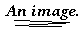
\includegraphics{image} \hfill 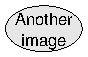
\includegraphics{image2}

Manually-added additional text.
\end{keyfigure}

The keyfigure is \cref{fig:keyfigure}.




\section{Keytable Environments}

\begin{keytable}{c=A keytable}
\testtable
\end{keytable}

\begin{keytable}{c=\dots continued,cont}
\testtable
\end{keytable}


\begin{keyfloats}{2}
\begin{keytable}{c=First keyfloats keytable,tc=centered}
\centering
\testtable
\end{keytable}
\begin{keytable}{c=Second keyfloats keytable}
\centering
\testwidetable
\end{keytable}
\begin{keytable}{c=Third keyfloats keytable}
\testtable
\end{keytable}
\begin{keytable}{c=\dots continued,cont}
\testwidetable
\end{keytable}
\end{keyfloats}

\begin{keysubtabs}{2}{c=Subtable Environments}
\begin{keytable}{c=First sub-keytable}
\testtable
\end{keytable}
\begin{keytable}{c=Second sub-keytable}
\testwidetable
\end{keytable}
\begin{keytable}{c=Third sub-keytable,tc=centered}
\centering
\testtable
\end{keytable}
\begin{keytable}{c=Fourth sub-keytable}
\testwidetable
\end{keytable}
\end{keysubtabs}

\begin{keysubtabs}{2}{cont,c={Subtable Environments, continued}}
\begin{keytable}{c=Fifth sub-keytable}
\testtable
\end{keytable}
\begin{keytable}{c=Sixth sub-keytable}
\testwidetable
\end{keytable}
\end{keysubtabs}



\clearpage

\section{One More Table}

\Cref{tab:onemore} is one more table.

\keytab{c=One More Table,l=tab:onemore}{\testtable}



\section{Keyfigbox and Keyparbox}

For a keyfigbox, w and lw keys control the width of the contents,
and thus also the width of the frame as well.

\keyfigbox{f,w=2in,c={A Keyfigbox 2in wide}}
	{\centering Some centered contents. \par Another paragraph. text text text text}

\keyfigbox[H]{lw=.75,f,r=15,c={A Keyfigbox [H] of .75 \cs{linewidth}}}
	{Some contents not centered. \par Another paragraph.
	text text text text text text text text text text text text text }

Following text.

\keyparbox{f,lw=1,t=A \cs{keyparbox} text and more text and more text and more text}{\raggedright text text text text text text text text  \par paragraph more more more more more more more more }


\begin{keyfloats}{2}
\keyparbox{f,lw=.5,t=A \cs{keyparbox} text and more text and more text and more text}{\raggedright text text text text text text text text  \par paragraph more more more more more more more more }
\keyparbox{f,lw=.75,t=\cs{keyparbox} 3/4 linewidth and more text and more text and more text}{\centering\huge\textbf{$\alpha$}}
\keyparbox{r=45,ft,w=.25in,tc=\cs{keyparbox} .25in and rotated}{\centering\textbf{$\beta$}}
\keyfig{f,lw=1,c=Next to keyfigboxes}{image}
\end{keyfloats}

\begin{keysubfigs}{2}{c=Subfigs and Parboxes}
\keyfig{c=A subfigure next to a parbox}{image}
\keyparbox{}{\centering A parbox, centered.}
\keyparbox{f}{A parbox, uncentered.}
\keyfig{c=Final subfig next to a parbox}{image2}
\end{keysubfigs}


\clearpage


\iffalse % Mixed subfloats lead to errors since subcaption v1.4d
\section{Mixed Subfloats}


\begin{keysubfigs}{4}{c=Mixed Subfloats,l=mixed:subfloats}
\keyfigbox{f,c=First mixed,l=mixed:first}{A keyfigbox.}
\keyfig{f,lw=1,c=Second mixed,l=mixed:second}{image}
\keytab{c=Third mixed,l=mixed:third}{\testwidetable}
\keyfig{lw=1,c=Fourth mixed,l=mixed:fourth}{image2}
\end{keysubfigs}




\begin{keysubfigs}{3}{
	c={\dots continued},l=mixed:contsubfloats,cont
}
\keytab{c=Fifth mixed,l=mixed:fifth}{\testtable}
\keyfig{lw=1,c=Sixth mixed,l=mixed:sixth}{image}
\keytab{c=Seventh mixed,l=mixed:seventh}{\testwidetable}
\end{keysubfigs}


The subfloats of \cref{mixed:subfloats} are
\cref{mixed:first}, \cref{mixed:second},
\cref{mixed:third}, and \cref{mixed:fourth}.


The continued subfloats of \cref{mixed:contsubfloats} are
\cref{mixed:fifth}, \cref{mixed:sixth}, and \cref{mixed:seventh}.

\textcolor{red}{Note: Each subfloat must be referred to as the same
type as its containing float.}
For example, a hypothetical subtable 3a inside figure 3 must be
referred to fig. 3a, even though it is a subtable,
so as to avoid mistaking for subtable of an entirely
different table 3.

\section{Yet Another Table}

Yet another table is \cref{tab:yetanother}
\keytab{w=.75in,c={Yet Another Table, Rotated},r=90,l=tab:yetanother}{\testtable}


\section{Mixed Subfloats as a Table}


\begin{keysubtabs}{3}{c=Mixed Subfloats as a Table,l=mixedtab:subfloats}
\keytab{c=First mixed table,l=mixedtab:first}{\testtable}
\keytab{c=Second mixed table,l=mixedtab:second}{\testwidetable}
\keyfig{lw=1,c=Associated Figure,l=mixedtab:third}{image}
\end{keysubtabs}

The subfloats of \cref{mixedtab:subfloats} are
\cref{mixedtab:first}, \cref{mixedtab:second}, and
\cref{mixedtab:third}.
\fi





\section{More Subtables}

\begin{keysubtabs}{2}{c=More Sub Tables,l=tab:moresubtables}
\keytab{c=First subtable,l=tab:morefirstsubtable}{\testtable}
\keytab{c=Second subtable,l=tab:moresecondsubtable}{\testtable}
\end{keysubtabs}

\begin{keysubtabs}{2}{c={\dots continued},l=tab:contmoresubtables,cont}
\keytab{c=Third subtable,l=tab:morethirdsubtable}{\testwidetable}
\keytab{w=1in,r=90,c={Fourth subtable, rotated},l=tab:morefourthsubtable}{\testwidetable}
\end{keysubtabs}

The subtables of \cref{tab:moresubtables} are
\crefrange{tab:morefirstsubtable}{tab:morefourthsubtable}.



\twocolumn[\section{Two-column mode}]

\setlength{\parskip}{0ex}
\setlength{\parindent}{2em}


\sloppy

\textcolor{red}{Note that floats may be placed out of order
when mixing single- and double-column floats
and when mixing [H] and non-[H] floats.}
They are included here for testing purposes.

Text before the unstarred keyfig.

\keyfig{,f,c={Unstarred Keyfig}}{image}

Text before the unstarred keytab.

\keytab{c=Unstarred keytab}{\testtable}

Text before the unstarred keyfig [H].

\keyfig[H]{f,c={Unstarred Keyfig [H]}}{image2}

Text before the unstarred keytab [H].

\keytab[H]{c=Unstarred keytab [H]}{\testtable}

Text before the starred keyfig.

\keyfig*{,c={Starred Keyfig}}{image}

Text before the starred keytab.

\keytab*{c=Starred keytab}{\testtable}

Text before the unstarred keyfloats.

\begin{keyfloats}{2}
\keyfig{,lw=1,c=Left Unstarred}{image}
\keyfig{lw=1,c=Right Unstarred}{image2}
\end{keyfloats}

Text before the unstarred keyfloats [H].

\begin{keyfloats}[H]{2}
\keyfig{f,lw=1,c=Left Unstarred [H]}{image}
\keyfig{lw=1,c=Right Unstarred [H]}{image2}
\end{keyfloats}

Text before the starred keyfloats.

\begin{keyfloats}*{2}
\keyfig{,lw=1,c=Left Starred}{image}
\keyfig{lw=1,c=Right Starred}{image2}
\end{keyfloats}

Text before the unstarred sub-figures.

\begin{keysubfigs}{2}{c=Unstarred Sub-Figures}
\keyfig{lw=1,f,c={Left Unstarred Subfigure}}{image}
\keyfig{lw=1,f,c={Right Unstarred Subfigure}}{image2}
\end{keysubfigs}

Text before the starred sub-figures.

\begin{keysubfigs}*{3}{c=Starred Sub-Figures}
\keyfig{lw=1,f,c={Left Starred Subfigure}}{image}
\keyfig{lw=1,f,c={Center Starred Subfigure}}{image2}
\keyfig{lw=1,f,c={Right Starred Subfigure}}{image}
\end{keysubfigs}

% \begin{keysubfigs}*{3}{c={Starred Sub-Figures, continued},sc={\dots\ continued},cont}
% \keyfig{lw=1,f,c={Left Starred Continued Subfigure}}
% \keyfig{lw=1,f,c={Center Starred Continued Subfigure}}{image2}
% \keyfig{lw=1,f,c={Right Starred Continued Subfigure}}
% \end{keysubfigs}

\keyflt{diagram}{
    f,
    aup=Mr.,
    auf=First,
    aul=Last,
    aus={~III},
    tc={About the diagram.},
    c=Two-column author,
}
{A diagram.}

\keyflt*{diagram}{
    f,
    aup=Mr.,
    auf=First,
    aul=Last,
    aus={~III},
    tc={About the diagram.},
    c=Two-column starred author,
}
{A starred diagram.}



Starred subfigures are sized relative to textwidth, but if they
are HERE in a two-column format then they placed into one column,
so it doesn't make much sense to combine star and [H].

\bigskip

\hrule

\lipsum


\onecolumn


\clearpage
% \newgeometry{inner=.5in,outer=2.5in,marginparwidth=2in}

\section{Margin Floats}

\begin{marginfigure}
\centering
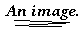
\includegraphics[width=.75\linewidth]{image}

Some text added by hand.
\caption{A \env{marginfigure}}
\label{fig:marginfigure}
\end{marginfigure}

\lipsum[1]

\begin{margintable}
\centering
\testwidetable
\caption{A \env{margintable}}
\label{fig:margintable}
\end{margintable}

\lipsum[2]

\keyfig[M]{c={A \cs{keyfig}\texttt{[M]}},l=fig:keyfigm,ft,
	t=Additional text.
	Text text text text text text.

	More paragraphs.
}{image2}

\lipsum[3]

\begin{keytable}[M]{
    c={A \env{keytable}\texttt{[M]}},
	l=tab:keytablem,mo=-.9in
}
\testwidetable
\end{keytable}

\lipsum[4]


\begin{keyfloats}[M]{2}
\keyfig{lw=1,f,c={First Keyfloats [M]},t=Some Text}{image}
\keyfig{lw=1,f,r=90,c={Second Keyfloats [M]},t=Lots of lots of lots of lots of text.}{image2}
\keytab{f,c={Third Keyfloats[M]},t=A table}{
\testtablethree
}
\end{keyfloats}
\blindtext[2]

\begin{keysubtabs}[M]{2}{c={Keysubtabs [M]}}
\keytab{f,c={First Keysubtabs[M]},t=A table}{\testtable}
\keytab{f,c={Second Keysubtabs[M]},t=Another table}{\testtable}
\end{keysubtabs}
\blindtext


\clearpage
\restoregeometry

\section{Wrapped Floats}

A simple wrapfigure:

\begin{wrapfigure}{r}{1in}
\fbox{Some text.}
\end{wrapfigure}
\blindtext

\keyfig[W]{c={A \cs{keyfig}\texttt{[W]}},
	l=fig:keyfigw,ft,lw=.4,wp=I,
	t={.4\cs{linewidth} wide, placed \texttt{I}.}
}{image2}
\blindtext

\keytab[W]{c={A \cs{keytab}\texttt{[W]}},l=tab:keytabw,w=.75in,
}{\testtable}
\blindtext[1]


\keyfigbox[W]{c={A \cs{keyfigbox}\texttt{[W]}},
	l=fig:keyfigboxw,f,lw=.25,wp=I,
	t=Text text text text text text text text text
}{The contents.}
\blindtext[1]

\keyparbox[W]{w=1in}{A \cs{keyparbox}[W] and some more text.}
\blindtext[1]

\begin{keyfigure}[W]{c={A \cs{keyfigure}\texttt{[W]}},
	l=fig:keyfigurew,f,w=1.5in}
This is a keyfigure.
\end{keyfigure}
\blindtext

\begin{keytable}[W]{c={A \env{keytable}\texttt{[W]}},
	l=tab:keytablew,w=2in,wp=L,tc=Placed \texttt{L} and 2in wide.}
\centering\testwidetable
\end{keytable}
\blindtext



\begin{itemize}
\item First item.
    Several lines of text text text text text
    text text text text text text text text.
\item \begin{keywrap}{.2\linewidth}{\keyfig{%
      lw=1,c={Keywrap with \cs{keyfig}},l=fig:keywrapfig%
    }{image}}
        Second item.
        Several lines of text text text text text
        text text text text text text text text text
        text text text text text text text.

        These paragraphs are inside the \texttt{keywrap}.
        A vertical gap appears below if the text is not enough to
        fill the space next to the \cs{keyfig}.
    \end{keywrap}
    Outside the \env{wrapfig},
    but still in the second item.
    There is no elegant way to place only part of a paragraph
    inside a \env{keywrap}, and attempting to do so requires
    manually removing the vertical paragraph skip.
\item Third item.
\end{itemize}


\clearpage

\begin{keyfloats}[W]{2}
\keyfig{lw=1,f,c={First Keyfloats [W]},t=Some Text}{image}
\keyfig{lw=1,f,r=90,c={Second Keyfloats [W]},t=Lots of lots of lots of lots of text.}{image2}
\keytab{f,c={Third Keyfloats[W]},t=A table}{\testtable}
\end{keyfloats}
\blindtext[2]

\begin{keysubfigs}[W]{2}{c={keysubfigs [W]}}
\keyfig{lw=1,f,c={First Subfigure [W]},t=Some Text}{image}
\keyfig{lw=1,f,c={Second Subfigure [W]},t=Lots of lots of lots of lots of text.}{image2}
\end{keysubfigs}
\blindtext



\clearpage

\begin{itemize}
\item First item.
\item \begin{keywrap}{.3\linewidth}{
\begin{keysubfigs}{2}{c={Keywrap keysubfigs}}
\keyfig{%
  f,lw=1,c={First wrapped \env{keysubfloat}}%
}{image}
\keyfig{%
  f,lw=1,c={Second wrapped \env{keysubfloat}}%
}{image2}
\end{keysubfigs}
}
\blindtext
\end{keywrap}
Outside the \env{wrapfig}:
\blindtext
\item Third item.
\item Fourth item.
\begin{keywrap}{.3\linewidth}{
\begin{keyfloats}{2}
\keyfig{%
  f,lw=1,c={First wrapped \env{keyfloats}}%
}{image}
\keyfig{%
  f,lw=1,c={Second wrapped \env{keyfloats}}%
}{image2}
\end{keyfloats}
}
\blindtext
\end{keywrap}
Outside the \env{wrapfig}.
\end{itemize}

\clearpage


\section{Spacing}

A sentence.
\keyfig{lw=.3}{image}
Another sentence.

A sentence.
\keyfigbox{lw=.3}{A keyfigbox.}
Another sentence.

A sentence.
\keyparbox{lw=.3}{A keyparbox /par Another paragraph.}
Another sentence.

A sentence.
\keytab{lw=.3}{\testtable}
Another sentence.

Before
\begin{keyfloats}{2}
\keytab{c=SubtableA}{\testtable}
\keytab{c=SubtableB}{\testtable}
\end{keyfloats}
after the keyfloats.

\begin{keysubtabs}{3}{c=Sub Tables A,l=tab:subtablesA}
\keytab{c=First subtable A,l=tab:firstsubtableA}{\testtable}
\keytab{c=Second subtable A,l=tab:secondsubtableA}{\testtable}
\keytab{f,t=(Framed),c=Third subtable A,l=tab:thirdsubtableA}{\testwidetable}
\keytab{c=Fourth subtable A,l=tab:fourthsubtableA}{\testwidetable}
\begin{keyfloats}{1}
\keytab{c=Fifth subtable A,l=tab:fifthsubtableA}{\testtable}
\keytab{c=Sixth subtable A,l=tab:sixthsubtableA}{\testtable}
\end{keyfloats}
\keytab{w=.75in,ft,r=15,tc=(Rotated and tightly framed.),c=Seventh subtable A,l=tab:seventhsubtableA}{\testtable}
\end{keysubtabs}

End of spacing section.

\clearpage

\section{Arbitrary float types}

Abitrary float types are here.

\keyflt{figure}{c=Arbitrary figure type}{%
    \fbox{An arbitrary figure float.}%
}

\keyflt[H]{figure}{c=Arbitrary figure type [H]}{%
    \fbox{An arbitrary figure float [H].}%
}

\keyflt[H]{figure}{c=Arbitrary figure type [H],lw=.3}{%
    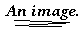
\includegraphics[width=\linewidth]{image}%
}



before the keyfloats
\begin{keyfloats}{2}
\keyflt{diagram}{
    c=A diagram macro,
    af=First,
    al=Last
}{%
    \fbox{An diagram float macro.}%
}
\begin{keyfloat}*{diagram}{
    c=A diagram environment,
    auf=First,
    aul=Last,
    t={Some text.  wert ewrt wertyerty ertyer yeruyty wer wqer qwer qwer
        wertert wertywety rtyeryer yrty wey erywe ty.

        eqrt werterqwt qert eqwrtertretwert.
    }
}
\fbox{A diagram environment.}

sf sadf asdf sdfg sdfgsdfg e rg ert ewrt erg sdfgasfd asdf asdf asdf asdf

sdfasdf sadf asdf asdf asdf asdfsdf sdf sadf asdfasdf saf asdf asdfasdfs sadfasdf
sadfsd fd sdf asdf sdfasdf
\end{keyfloat}
\end{keyfloats}
after the keyfloats


before the keysubfloats
\begin{keysubfloats}{diagram}{2}{
    c=Diagram subfloats
}
\keyflt{diagram}{
    c=A sub diagram macro,
    af=First,
    al=Last
}{%
    \fbox{An diagram subfloat macro.}%
}
\begin{keyfloat}*{diagram}{
    c=A sub diagram environment,
    af=First,
    al=Last,
    l=dia:subtwo
}
\fbox{A diagram subfloat environment.}
\end{keyfloat}
\end{keysubfloats}
after the keysubfloats

The second subdiagram is ref \ref{dia:subtwo} and cref \cref{dia:subtwo}.


\keyflt{diagram}{c=\cs{keyflt} diagram}{%
    \fbox{A \cs{keyflt} diagram.}%
}

\keyflt[W]{diagram}{lw=.3,c=Wrapped \cs{keyflt} diagram}{%
    A wrapped \cs{keyflt} diagram.%
}
\blindtext

\keyflt[M]{diagram}{f,c=Margin \cs{keyflt} diagram}{%
    A margin \cs{keyflt} diagram.%
}
\blindtext



\begin{keyfloat}[W]{diagram}{
    c={A diagram \cs{keyfloat}\texttt{[W]}},
    l=fig:keyfloatw,f,w=1.5in}
This is a diagram keyfloat.
\end{keyfloat}
\blindtext

\noindent\begin{keywrap}{1.25in}{
    \keyflt{diagram}{
        c=A wrapped diagram,
        af=First,
        al=Last,
        w=1in
    }{%
        A wrapped diagram float macro.
    }
}
% \noindent% *88*
\blindtext
\end{keywrap}
\blindtext


the margin float is here

\begin{keyfloat}[M]{diagram}{
    c={A diagram \cs{keyfloat}\texttt{[M]}},
    l=fig:keyfloatm,f,
}
This is a margin diagram keyfloat.
\end{keyfloat}

\lipsum[2]

Between

\begin{keyfloat}[H]{diagram}{
    c={A diagram \cs{keyfloat}\texttt{[H]}},
    l=fig:keyfloath,f,
}
This is a [H] diagram keyfloat.
\end{keyfloat}




% % To test an invalid float type:
% \keyflt{xyz}{c=Arbitrary figure type}{
% \fbox{An arbitrary figure float.}
% }

% % To test keyflt used as an environment:
% \begin{keyflt}{figure}{c=Arbitrary figure type}
% blarg
% \end{keyflt}

End of arbitrary float types.

\clearpage

\section{Figurehere and Tablehere}

A figurehere follows:
\begin{figurehere}
\centering
\fbox{Inside a figurehere.}
\caption{A figurehere}
\end{figurehere}

A tablehere follows:
\begin{tablehere}
\centering
\caption{A tablehere}
\fbox{Inside a tablehere.}
\end{tablehere}


\clearpage

\section{Artists}

\keyfig{
    f,
    c=With an artist,
    l=fig:artist,
    ap=Mr.,af=First,al=Last,as={, Artist},
}{image2}

\Cref{fig:artist} has an artist.


\keyfig{
    c=With an artist and text,
    l=fig:artisttext,
    ap=Mr.,af=First,al=Last,as={, Artist},
    t={some text}
}{image2}

\Cref{fig:artisttext} has an artist and text.


\section{Authors}

\keyflt[H]{diagram}{
    f,
    aup=Mr.,
    auf=First,
    aul=Last,
    aus={~III},
    t={About the illustration.},
    c=Artist's name — image,
    l=fig:author
}
{A diagram. sdf sad f asdf asdf as df asdf asd f asdf asdf as df asdf asd f}




\end{document}
